\documentclass[]{scrartcl}
\usepackage{graphicx}
\usepackage{geometry}
\geometry{
	a4paper,
	total={170mm,257mm},
	left=20mm,
	top=20mm,
}


%opening
\title{SDD -Hearts Low Level Design}
\author{Brandon Smith, Nieka Gutenberger, Joseph Coppin, Ryan Frazier, Trevor Jewkes}

\begin{document}

\maketitle

\centerline{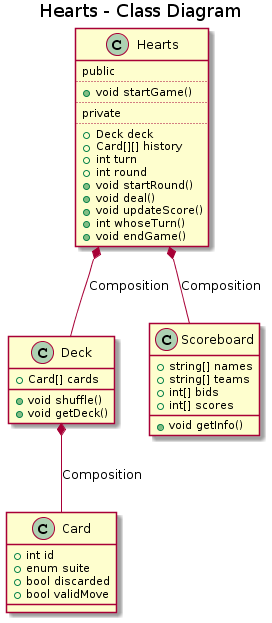
\includegraphics{Hearts_Class_diagram.png}}
\centerline{Hearts Low Level Design Diagram}

\section{Hearts Class}



\subsection{std::string suite(int i)}  
	converts enum ints to string of suit
\subsection{std::vector $\langle$Card$\rangle$ initializeDeck()} 
	creates deck of cards taken from Card.cpp
\subsection{std::string makename(int n) } 
	converts Player + int into Player names
\subsection{std::vector$\langle$Player$\rangle$  creatPlayers(int p) } 
	Creats a vector of Players to play the game.
\subsection{std::string value(int i)}
\subsection{void displayCards(std::vector$\langle$Card$\rangle$ \& hand)}
	displays the deck for screen purposes.
\subsection{void dealCards(std::vector$\langle$Player$\rangle$ \& players, std::vector$\langle$Card$\rangle$ \& Deck)}
\subsection{int findTwoOfClubs(std::vector$\langle$Player$\rangle$ \& p)}  
	looks through each hand to find the 2 of clubs
\subsection{Card getCardsToPass(std::vector$\langle$Card$\rangle$ \& h, std::string p) }
	gets and stores cards for passing
\subsection{int fixPass(int r, int p, int c)}
\subsection{void assignPassedCards(std::vector$\langle$Player$\rangle$ \& p, std::vector$\langle$Card$\rangle$ \& h, int r)  }
	takes the passed cards and redistributes based on round
\subsection{int passCards(std::vector$\langle$Player$\rangle$ \& p, int round)  }
	function for passing cards at beginging of round
\subsection{int scoretrick(std::vector$\langle$Card$\rangle$ \& center, std::vector$\langle$Player$\rangle$ \& players, int\& turn)}
\subsection{void displayroundScores(std::vector$\langle$Player$\rangle$ p)}
\subsection{void displayScores(std::vector$\langle$Player$\rangle$  p)}
\subsection{bool allhearts(std::vector$\langle$Card$\rangle$ h)  }
	checks to see if a players hand is all hearts.
\subsection{bool noLeadSuit(Suit s, std::vector$\langle$Card$\rangle$ h) }
	 compares hand against the lead suit
\subsection{bool validateMove(Player\& p, bool\& broken, std::vector$\langle$Card$\rangle$  Center, Card move, int t, int i)}
\subsection{Card getmove(Player\& p, bool\& b, std::vector$\langle$Card$\rangle$  c, int t, int i)}
\subsection{void updateScore(std::vector$\langle$Player$\rangle$ \& p)}
	adds round score to Score
\subsection{bool playRound(std::vector$\langle$Player$\rangle$ \& players, std::vector$\langle$std::vector$\langle$Card$\rangle$ $\rangle$\& history, int round)}
\subsection{void startGame(std::vector$\langle$Player$\rangle$ \& players, std::vector$\langle$std::vector$\langle$Card$\rangle$ $\rangle$\& history) }
	 uses players and calls round until game is over
\subsection{void play\_Hearts(int num)}



\end{document}
